\documentclass{standalone}
\usepackage{pgfplots}
\begin{document}
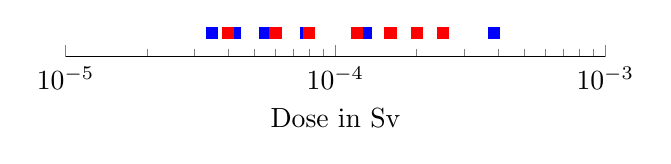
\begin{tikzpicture}
\begin{axis}[
    y=1.5cm,            % y unit vector
    hide y axis,        % hide the y axis
    xmode = log,        % logarithmic x axis
    axis x line*=bottom,% only show the bottom x axis line, without an arrow tip
    xmin=1e-5, xmax=1e-3,% range for the x axis
    xlabel = Dose in Sv
]
\addplot [only marks, mark=square*, fill=blue , draw=blue] table {
3.86e-4 1
1.30e-4 1
7.76e-5 1
5.48e-5 1
4.24e-5 1
3.48e-5 1
};
\addplot [only marks, mark=square*, fill=red , draw=red] table {
40e-6 1
60e-6 1
80e-6 1
120e-6 1
160e-6 1
200e-6 1
250e-6 1
};
\end{axis}
\end{tikzpicture}

\end{document}